\chapter[Apéndice: Manual de usuario]{
  \label{chp:usermanual}
  Manual de usuario
}

Neste apéndice apórtase un manual de referencia para os usuarios da web.

\begin{figure}[h]
	\centering
	\fbox{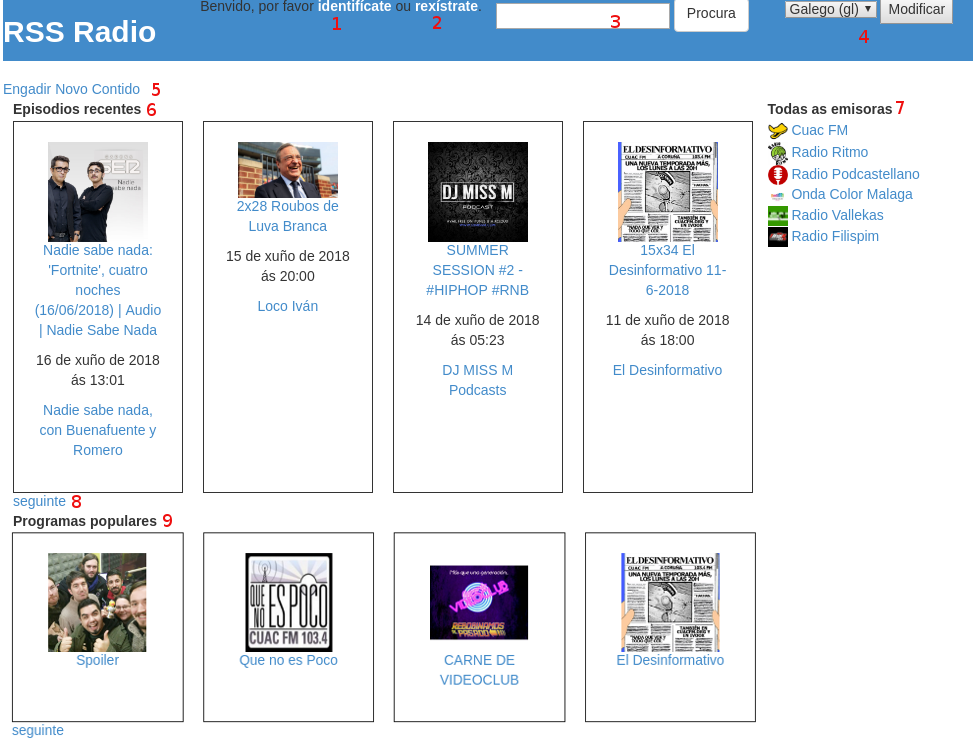
\includegraphics[scale=0.4,keepaspectratio=true]{./images/usermanual/um-index-anon.png}}
	\caption{Portada da web para usuario anónimo}
	\label{fig:um-index-anon}
\end{figure}

Na figura \ref{fig:um-index-anon} amósase o aspecto da portada da web para un usuario anónimo con números identificando as distintas áreas:

\begin{itemize}
	\item \textbf{1:} Enlace á páxina de login.
	\item \textbf{2:} Enlace á páxina de rexistro.
	\item \textbf{3:} Caixa de procura por texto.
	\item \textbf{4:} Selector de idioma.
	\item \textbf{5:} Enlace ao menú de creación de novo programa e emisora. Require identificación.
	\item \textbf{6:} Sección de episodios recentes. Amósanse os 4 últimos episodios engadidos ao sistema independentemente do seu programa. Para ver os 4 seguintes, pódese premer o botón marcado co \textbf{8}.
	\item \textbf{7:} Lista de emisoras presentes no sistema.
	\item \textbf{8:} Botón para cargar a seguinte páxina.
	\item \textbf{9:} Sección de programas ordenados por popularidades. Amósanse os 4 primeiros tamén con opción de cargar a seguinte páxina.  
\end{itemize}